\begin{figure}
  \centering

  \begin{subfigure}{\linewidth}
    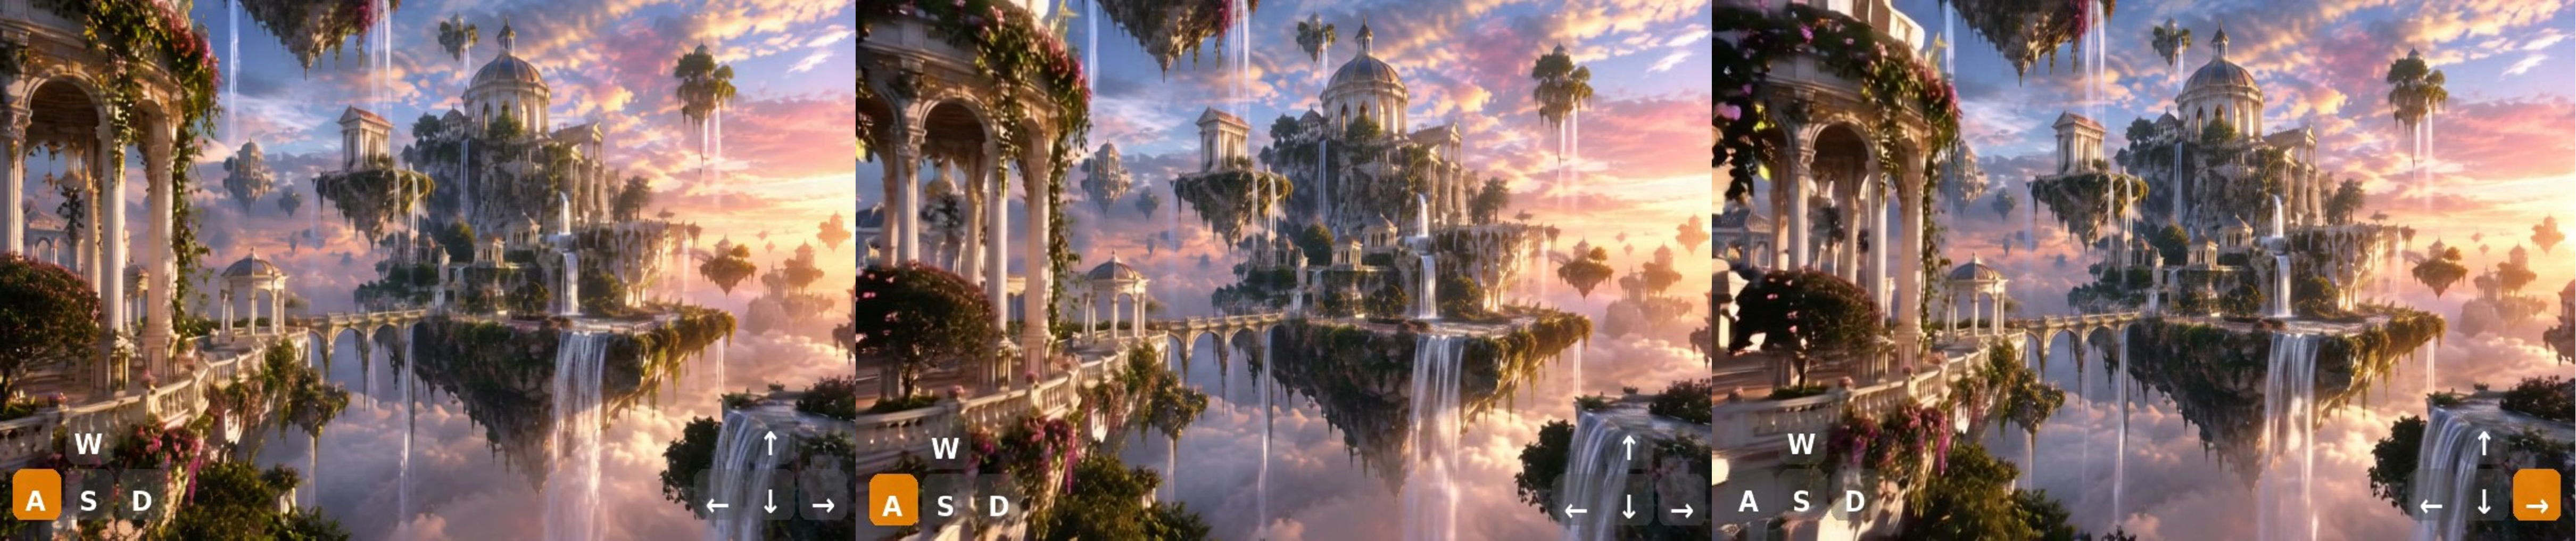
\includegraphics[width=\linewidth]{Figures/bs-a.pdf}
    \caption{\textbf{Training with very small batch sizes.}
    When the batch size is smaller than 4, the Wan2.1-based model often fails to learn camera-controllable generation.}
  \end{subfigure}

  \vspace{0.5em}

  \begin{subfigure}{\linewidth}
    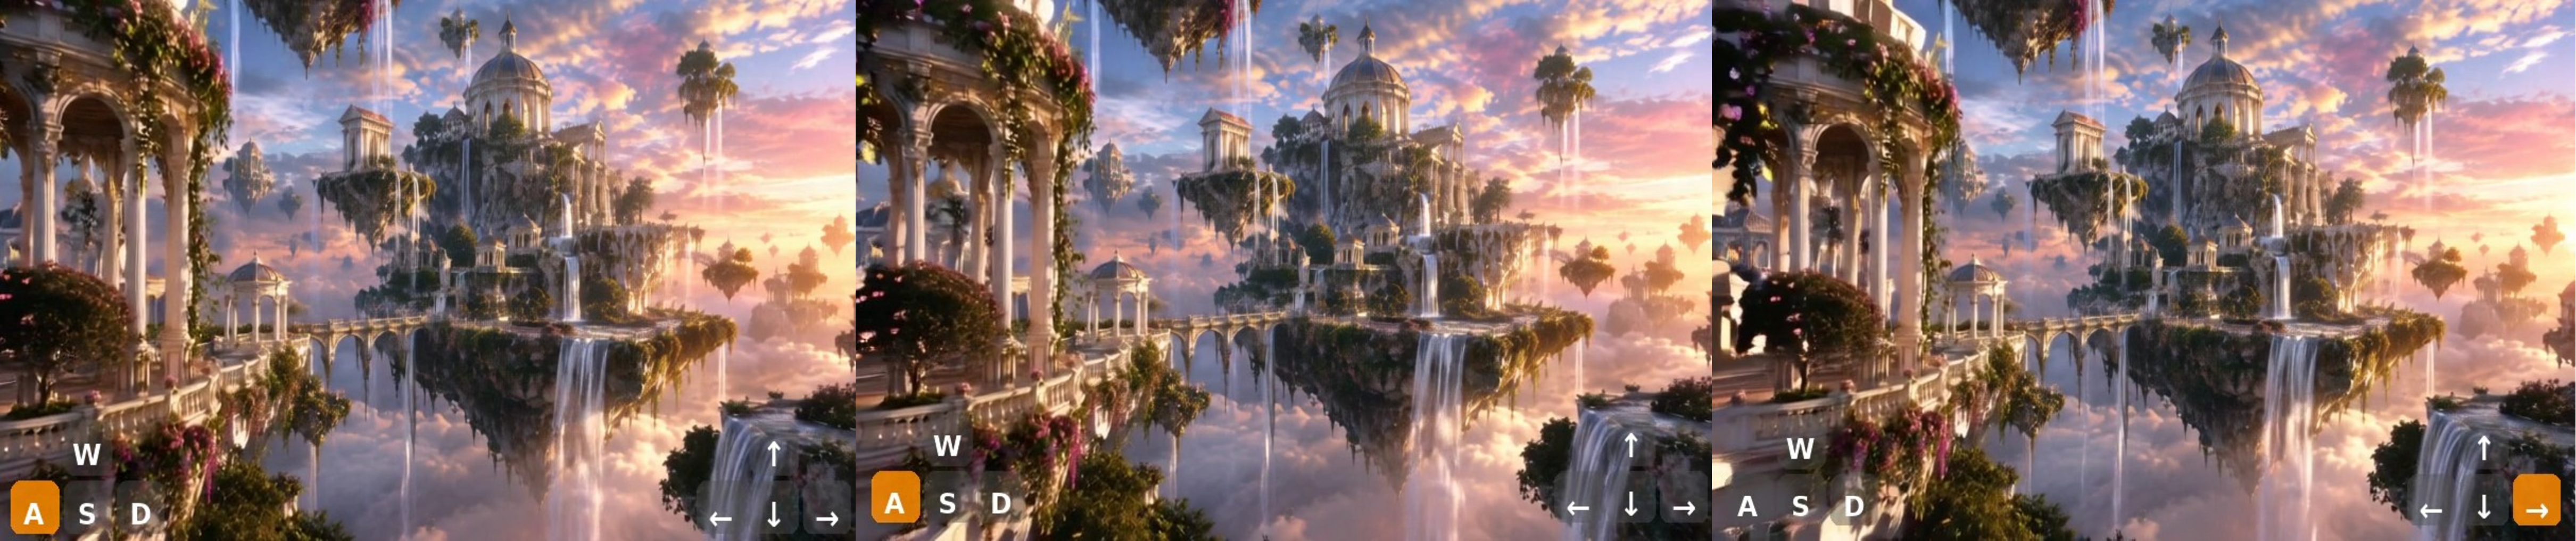
\includegraphics[width=\linewidth]{Figures/bs-b.pdf}
    \caption{\textbf{Training with batch size 8.}
    With a batch size of 8, the model's controllability improves substantially, but remains somewhat unstable.}
  \end{subfigure}

  \vspace{0.5em}

  \begin{subfigure}{\linewidth}
    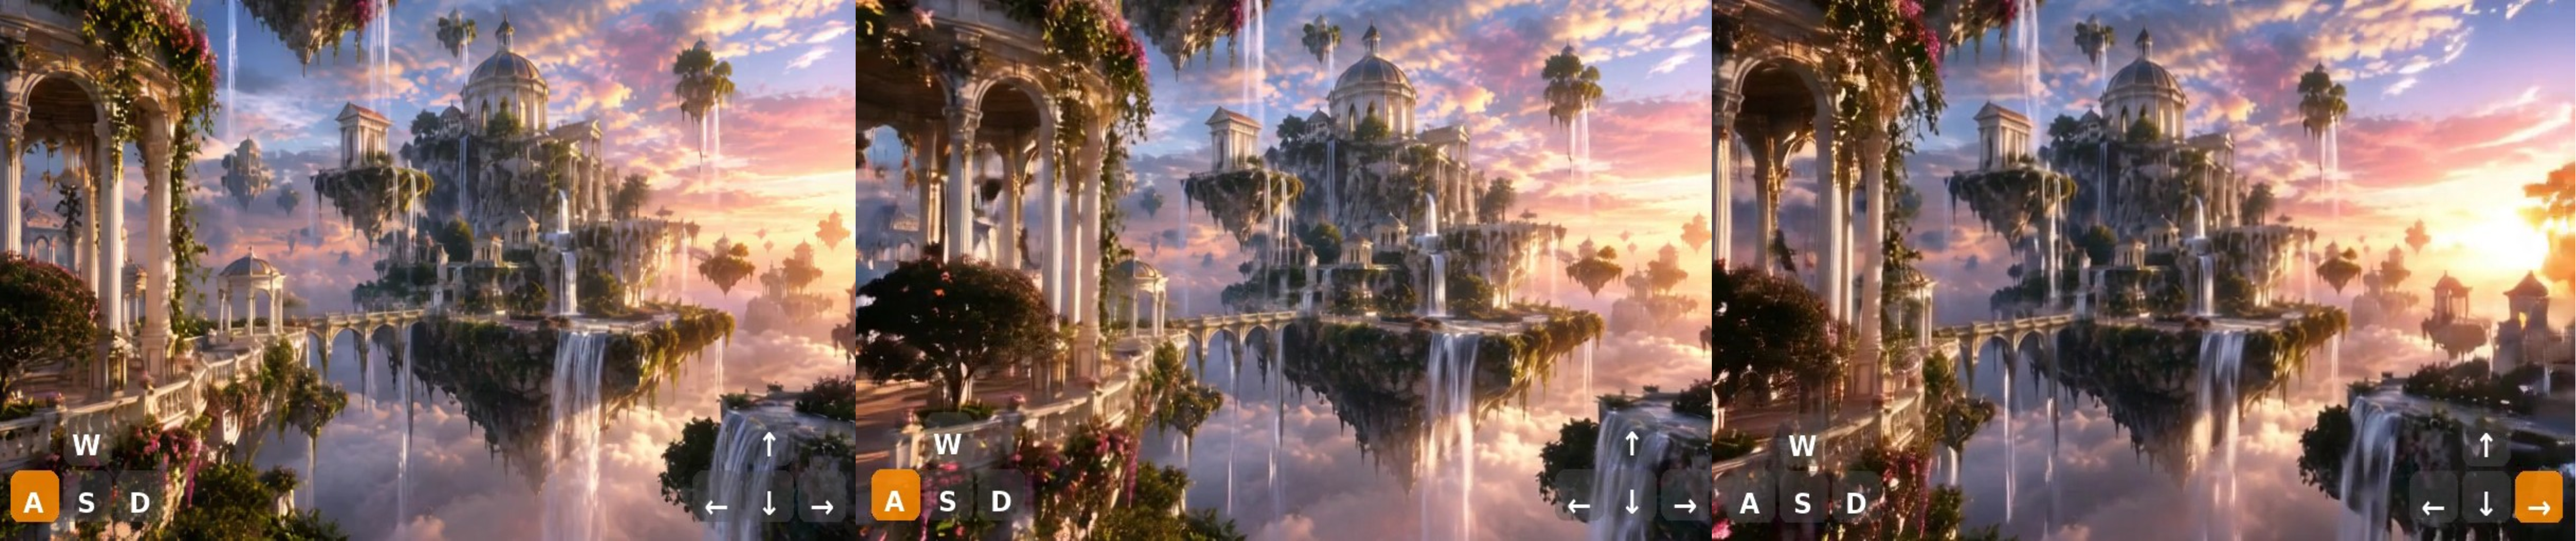
\includegraphics[width=\linewidth]{Figures/bs-c.pdf}
    \caption{\textbf{Training with batch size 16.}
    With a batch size of 16, the full training pipeline can be successfully completed with high controllability.}
  \end{subfigure}

  \caption{\textbf{Effect of batch size on camera-controllable generation.}
  Using Wan2.1 as an example, we find that batch size critically affects camera-control training: batch sizes below 4 often fail to learn controllability, batch size 8 substantially improves controllability but remains unstable, while batch size 16 enables successful training with high controllability.}
  \label{fig:ablation-bs}

\end{figure}